\chapter{Súčasný stav riešenej problematiky doma a v zahraničí}

V tejto kapitole sa zameriavame na teoretické a metodologické východiská symetrického problému obchodného cestujúceho a na hlavné smery jeho súčasného riešenia. Pozornosť venujeme najmä prechodu od klasických optimalizačných prístupov k dátovo riadeným metódam, ktoré využívajú neurónové siete a grafové reprezentácie. Keďže práca je orientovaná na modelovanie nad hranami úplného grafu, štruktúra kapitoly je prispôsobená práve tým aspektom problému, ktoré sú relevantné pre edge-based formuláciu, syntetické tréningové dáta, benchmarkové hodnotenie a interpretáciu výsledkov.

\section{Teoretické východiská problému obchodného cestujúceho}

Problém obchodného cestujúceho (Traveling Salesman Problem, TSP) patrí medzi najznámejšie úlohy kombinatorickej optimalizácie. V základnej formulácii je daná množina miest a náklady presunu medzi každou dvojicou miest, pričom cieľom je určiť takú uzavretú trasu, ktorá navštívi každé mesto práve raz a minimalizuje celkové náklady. Napriek relatívne jednoduchej formulácii ide o úlohu s vysokou výpočtovou náročnosťou, ktorá sa dlhodobo používa ako referenčný problém pri porovnávaní presných algoritmov, heuristík, metaheuristík aj moderných prístupov založených na strojovom učení.

Takto formulovaný problém možno interpretovať ako úlohu na úplnom grafe $G=(V,E)$, v ktorom vrcholy reprezentujú mestá a hrany náklady alebo vzdialenosti medzi nimi. Hľadaným riešením je hamiltonovský cyklus s minimálnou celkovou cenou. Táto grafová interpretácia je dôležitá nielen z hľadiska matematickej formulácie, ale aj z pohľadu návrhu algoritmov, pretože umožňuje priamo pracovať so štruktúrou vrcholov, hrán a susedností.

\begin{figure}[htbp]
    \centering
    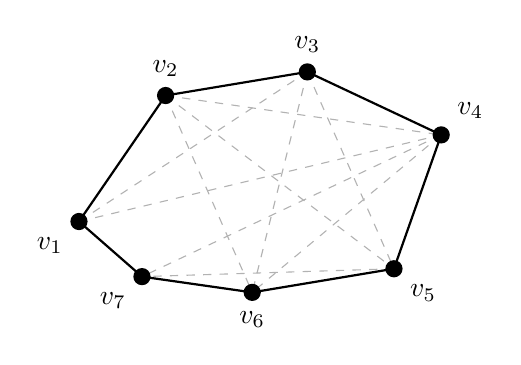
\begin{tikzpicture}[
    city/.style={circle, fill=black, inner sep=2.2pt},
    route/.style={thick},
    alt/.style={gray!60, thin, dashed}
]

\coordinate (A) at (0.2,1.1);
\coordinate (B) at (1.3,2.7);
\coordinate (C) at (3.1,3.0);
\coordinate (D) at (4.8,2.2);
\coordinate (E) at (4.2,0.5);
\coordinate (F) at (2.4,0.2);
\coordinate (G) at (1.0,0.4);

% pomocné spojenia
\draw[alt] (A)--(C);
\draw[alt] (A)--(D);
\draw[alt] (B)--(D);
\draw[alt] (B)--(E);
\draw[alt] (C)--(E);
\draw[alt] (C)--(F);
\draw[alt] (D)--(F);
\draw[alt] (D)--(G);
\draw[alt] (E)--(G);
\draw[alt] (B)--(F);

% výsledná trasa
\draw[route] (A)--(B)--(C)--(D)--(E)--(F)--(G)--(A);

% vrcholy
\node[city,label=below left:$v_1$] at (A) {};
\node[city,label=above:$v_2$] at (B) {};
\node[city,label=above:$v_3$] at (C) {};
\node[city,label=above right:$v_4$] at (D) {};
\node[city,label=below right:$v_5$] at (E) {};
\node[city,label=below:$v_6$] at (F) {};
\node[city,label=below left:$v_7$] at (G) {};

\end{tikzpicture}
    \caption{Ilustračná euklidovská inštancia symetrického problému obchodného cestujúceho s vyznačenou výslednou trasou.}
    \label{fig:tsp_instance}
\end{figure}

Z tejto základnej formulácie vychádza viacero variantov problému TSP, ktoré sa odlišujú najmä vlastnosťami nákladovej matice, počtom obchodných cestujúcich alebo prítomnosťou dodatočných obmedzení. Medzi najčastejšie uvádzané varianty patria:

\begin{itemize}[leftmargin=1.5cm,itemsep=3pt,topsep=4pt]
    \item \textbf{STSP (Symmetric Traveling Salesman Problem),} pri ktorom je náklad presunu z vrcholu $i$ do vrcholu $j$ rovnaký ako náklad v opačnom smere;
    \item \textbf{ATSP (Asymmetric Traveling Salesman Problem),} v ktorom sa náklady presunu môžu líšiť podľa smeru pohybu;
    \item \textbf{mTSP (Multiple Traveling Salesman Problem),} kde je úloha rozdelená medzi viacerých obchodných cestujúcich;
    \item \textbf{TSPTW (Traveling Salesman Problem with Time Windows),} pri ktorom musia byť jednotlivé vrcholy navštívené v určených časových intervaloch;
    \item \textbf{viackriteriálne varianty TSP,} v ktorých sa optimalizácia nevzťahuje iba na jednu cieľovú funkciu, ale súčasne napríklad na čas, náklady alebo riziko.
\end{itemize}

Jednotlivé varianty vznikli ako reakcia na praktické požiadavky v logistike, plánovaní výroby, skladovaní, rozvoze alebo v navigačných systémoch. Hoci sa medzi sebou líšia konkrétnymi obmedzeniami, všetky vychádzajú z rovnakého princípu: nájsť efektívne poradie návštevy viacerých bodov pri rešpektovaní definovaných pravidiel úlohy.

V tejto práci sa zameriavame na symetrický problém obchodného cestujúceho. V tomto variante platí, že náklad presunu z vrcholu $i$ do vrcholu $j$ je rovnaký ako náklad presunu z vrcholu $j$ do vrcholu $i$. STSP predstavuje klasickú a metodologicky dobre preskúmanú formuláciu, ktorá sa často používa ako základ pri porovnávaní algoritmov, benchmarkových inštancií a metrík hodnotenia. Zároveň ide o variant, ktorý je vhodný aj pre experimentálne porovnávanie dátovo riadených modelov, keďže umožňuje pracovať s jednotnou a dobre interpretovateľnou štruktúrou úlohy.

Význam TSP však nespočíva iba v jeho teoretickej elegancii. Problém má široké praktické uplatnenie v logistike, distribúcii, plánovaní servisných trás, sekvenovaní výrobných operácií, návrhu dosiek plošných spojov, bioinformatike či v konštrukcii testovacích úloh pre nové optimalizačné postupy. Práve spojenie jasnej matematickej definície, praktickej relevancie a vysokej výpočtovej náročnosti vysvetľuje, prečo TSP zostáva dlhodobo jednou z centrálnych úloh operačného výskumu.

\section{Výpočtová náročnosť a klasické prístupy k riešeniu}

Na riešenie problému obchodného cestujúceho bolo navrhnuté široké spektrum prístupov, ktoré sa postupne vyvíjali v závislosti od požiadaviek na presnosť, rýchlosť a praktickú použiteľnosť. V tejto časti sa zameriavame na vysvetlenie výpočtovej náročnosti problému a na hlavné skupiny klasických metód používaných pri jeho riešení.

\noindent\textbf{Výpočtová náročnosť problému.}

Problém obchodného cestujúceho patrí medzi výpočtovo náročné optimalizačné úlohy. Jednoducho povedané to znamená, že počet možných trás rastie s počtom vrcholov veľmi rýchlo, a preto už pri stredne veľkých inštanciách nie je možné ani efektívne, ani časovo prijateľné úplne prehľadať priestor všetkých riešení. V prípade symetrického TSP je počet rôznych cyklov rádovo $(n-1)!/2$, čo dobre ilustruje, prečo sa problém s rastúcim počtom miest stáva prakticky neriešiteľným úplným prehľadaním priestoru riešení.

Práve táto vlastnosť mala zásadný vplyv na vývoj metód riešenia. Ukázalo sa, že pri menších inštanciách možno hľadať optimálne riešenie pomocou presných algoritmov, no pri väčších úlohách je potrebné pracovať s prístupmi, ktoré uprednostňujú rýchlosť a praktickú použiteľnosť pred garanciou absolútneho optima. Z historického aj metodologického hľadiska sa preto vyprofilovali dve hlavné skupiny klasických prístupov: presné metódy a heuristické, resp. metaheuristické postupy.

\noindent\textbf{Presné metódy riešenia.}

Presné metódy sú zamerané na nájdenie garantovane optimálneho riešenia. Medzi najdôležitejšie prístupy v tejto skupine patria celočíselné lineárne formulácie, vetvenie a medze, vetvenie s rezmi či dynamické programovanie. Ich spoločným znakom je to, že pri splnení výpočtových podmienok umožňujú určiť skutočne najlepšiu možnú trasu, a preto predstavujú dôležitý referenčný základ pri hodnotení kvality iných algoritmov.

Význam presných metód nespočíva iba v samotnom riešení menších alebo stredne veľkých inštancií. Ich výsledky zohrávajú dôležitú úlohu aj pri benchmarkingu, pretože poskytujú referenčné hodnoty, voči ktorým možno porovnávať približné a dátovo riadené prístupy. Zároveň slúžia ako zdroj kvalitných štítkov pri tvorbe trénovacích množín, keďže práve optimálne alebo takmer optimálne riešenia umožňujú učiť modely na spoľahlivých cieľových výstupoch.

Nevýhodou presných metód je ich vysoká výpočtová náročnosť, ktorá sa prejavuje najmä pri rastúcej veľkosti inštancie. V praxi sa preto využívajú najmä tam, kde je potrebná garancia optimálnosti, alebo tam, kde je možné akceptovať vyššie časové a výpočtové náklady výmenou za maximálnu presnosť výsledku.

\noindent\textbf{Heuristiky a metaheuristiky.}

V situáciách, keď presné riešenie nie je časovo alebo výpočtovo realistické, sa uplatňujú heuristiky a metaheuristiky. Heuristické metódy konštruujú riešenie pomocou relatívne jednoduchých rozhodovacích pravidiel, napríklad postupným výberom najbližšieho suseda alebo vkladaním ďalších vrcholov do už vytváranej trasy. Ich hlavnou výhodou je rýchlosť a implementačná jednoduchosť, no spravidla neposkytujú garanciu optimálnosti a bývajú citlivé na lokálne rozhodnutia urobené v počiatočných krokoch.

Metaheuristiky predstavujú všeobecnejší rámec, v ktorom sa kombinuje konštrukcia riešenia s mechanizmami zlepšovania, diverzifikácie a vyhľadávania v priestore alternatívnych trás. Patria sem napríklad simulované žíhanie, tabu search, genetické algoritmy, mravčie kolónie alebo iteratívne lokálne prehľadávanie. Ich cieľom nie je nájsť garantované optimum, ale dosiahnuť čo najkvalitnejšie riešenie v prijateľnom čase.

V kontexte symetrického TSP zohrávajú osobitnú úlohu lokálne zlepšovacie techniky typu $k$-opt a heuristika Lin--Kernighan. Práve tieto prístupy ukázali, že aj bez formálnej garancie optimálnosti možno v praxi dosahovať veľmi kvalitné riešenia, ktoré sú často dostatočné pre reálne aplikácie aj pre experimentálne porovnávanie algoritmov.

\noindent\textbf{Význam klasických prístupov pre súčasný výskum.}

Klasické metódy riešenia TSP dnes nepredstavujú iba historický základ výskumu, ale stále zohrávajú dôležitú úlohu aj v súčasných prístupoch. Presné algoritmy poskytujú referenčné riešenia a heuristiky a metaheuristiky ostávajú praktickými nástrojmi na riešenie väčších inštancií. Navyše sa ukazuje, že mnohé moderné dátovo riadené a neurónové modely tieto klasické postupy nenahrádzajú úplne, ale skôr na ne nadväzujú.

V hybridných riešeniach sa napríklad model strojového učenia používa na predikciu sľubných hrán alebo na usmernenie prehľadávania, zatiaľ čo samotná výsledná trasa vzniká až pomocou heuristického dekódovania alebo následného lokálneho dolaďovania. Z toho vyplýva, že pochopenie klasických prístupov je nevyhnutné nielen pre teoretické uchopenie problému, ale aj pre správnu interpretáciu moderných výsledkov. Práve na tento vývoj prirodzene nadväzuje nasledujúca časť práce, ktorá sa venuje dátovo riadeným a neurónovým prístupom k riešeniu TSP.

\begin{figure}[htbp]
    \centering
    \begin{tikzpicture}[
    node distance=1.4cm and 1.6cm,
    box/.style={
        draw,
        rounded corners,
        align=center,
        minimum width=3.2cm,
        minimum height=0.95cm
    },
    arrow/.style={-{Latex[length=2.5mm]}, thick}
]

\node[box] (tsp) {Prístupy k riešeniu TSP};

\node[box, below left=of tsp] (exact) {Presné\\ metódy};
\node[box, below=of tsp] (heur) {Heuristiky a\\ metaheuristiky};
\node[box, below right=of tsp] (ml) {Dátovo riadené\\ prístupy};
\node[box, below=of heur] (hybrid) {Hybridné\\ prístupy};

\draw[arrow] (tsp) -- (exact);
\draw[arrow] (tsp) -- (heur);
\draw[arrow] (tsp) -- (ml);
\draw[arrow] (heur) -- (hybrid);
\draw[arrow] (ml) -- (hybrid);

\end{tikzpicture}
    \caption{Prehľad hlavných skupín prístupov k riešeniu problému obchodného cestujúceho.}
    \label{fig:tsp_methods}
\end{figure}

\section{Formulácia problému TSP pre dátovo riadené modely}

Pri klasickom riešení problému obchodného cestujúceho sa optimálna trasa hľadá priamo pomocou optimalizačného algoritmu. V prípade dátovo riadených prístupov je však potrebné túto úlohu najskôr previesť do podoby, s ktorou môže pracovať model strojového učenia. To znamená, že problém už nie je chápaný iba ako hľadanie najlepšej trasy, ale aj ako úloha nad dátami, v ktorej treba definovať vstupné inštancie, cieľové výstupy a vhodnú reprezentáciu riešenia.

Vstup do modelu zvyčajne tvorí množina vrcholov reprezentovaných súradnicami, maticou vzdialeností alebo odvodenými príznakmi hrán. Samotné vstupné inštancie však na učenie nestačia. Model potrebuje aj referenčné riešenia, na základe ktorých sa vytvoria cieľové štítky. V prípade TSP môže mať takýto štítok podobu celej optimálnej alebo približne optimálnej trasy, prípadne informácie o tom, ktoré hrany patria do referenčného riešenia.

Pri dátovo riadených prístupoch sa preto často využívajú synteticky generované inštancie, najmä euklidovské úlohy, pri ktorých sú vrcholy vytvorené náhodne v dvojrozmernom priestore. Výhodou takéhoto postupu je možnosť pripraviť veľké množstvo tréningových príkladov s kontrolovanou veľkosťou a štruktúrou. Zároveň však vzniká otázka kvality referenčných riešení. Presné riešiče poskytujú kvalitné štítky, ich použitie je však časovo a výpočtovo náročné. Aproximačné postupy sú rýchlejšie, no model sa pri nich učí z riešení, ktoré nemusia byť optimálne. Voľba medzi presnosťou štítkov a náročnosťou ich prípravy preto predstavuje dôležitý metodologický aspekt.

Pri návrhu modelu možno TSP formulovať viacerými spôsobmi. Jednou z možností je sekvenčné generovanie poradia vrcholov. Druhou, z pohľadu našej práce kľúčovou možnosťou, je formulácia problému ako predikcie hrán v úplnom grafe. V tomto prípade model nepredikuje priamo celé poradie miest, ale odhaduje, ktoré hrany sú dôležité pre výslednú trasu. Takáto formulácia je prirodzená preto, že samotný TSP je definovaný na grafe a riešenie možno chápať ako množinu hrán tvoriacich hamiltonovský cyklus.

Výhodou predikcie hrán je, že umožňuje pracovať s grafovou štruktúrou úlohy a s príznakmi odvodenými zo vzdialeností, geometrie alebo lokálneho usporiadania vrcholov. Z pohľadu učenia sa každá hrana stáva samostatnou jednotkou predikcie, pre ktorú model odhaduje skóre, pravdepodobnosť alebo triedu. Výstupom ešte nie je finálna trasa, ale štruktúrovaná informácia o tom, ktoré spojenia sú pre kvalitné riešenie perspektívne.

Dôležitým špecifikom tohto prístupu je, že samotná predikcia ešte nezaručuje vznik realizovateľného riešenia. Model môže priradiť vysoké skóre hranám, ktoré spolu nevytvárajú uzavretý cyklus spĺňajúci všetky podmienky TSP. Preto je medzi výstupom modelu a finálnou trasou nevyhnutná dekódovacia fáza, ktorá prevedie predikované skóre na konkrétny hamiltonovský cyklus. Táto fáza môže byť doplnená aj o lokálne zlepšovanie, čo vedie k hybridnému pipeline spájajúcemu dátovo riadený model s klasickými algoritmickými postupmi.

Pre potreby tejto práce má takáto formulácia zásadný význam, keďže umožňuje prepájať grafovú štruktúru TSP, prípravu tréningových dát a výstup neurónových modelov v jednotnom experimentálnom rámci. Práve na tomto základe následne stojí aj nasledujúca časť kapitoly, ktorá sa venuje konkrétnym dátovo riadeným a neurónovým prístupom k riešeniu TSP.

\section{Dátovo riadené a neurónové prístupy k riešeniu TSP}

V súčasnom výskume kombinatorickej optimalizácie sa čoraz väčšia pozornosť venuje prístupom, ktoré využívajú strojové učenie na odhad rozhodnutí vedúcich ku kvalitným riešeniam. Pri probléme obchodného cestujúceho to znamená, že model sa neučí priamo „riešiť“ úlohu v tradičnom zmysle, ale odhaduje štruktúrne vzory, ktoré možno následne využiť pri konštrukcii výslednej trasy. V našej práci sa zameriavame na taký typ dátovo riadených modelov, ktorý pracuje s hranami úplného grafu a hodnotí ich význam pre výsledné riešenie.

\noindent\textbf{Edge-based prístup ako základ modelovania.}

Pri edge-based formulácii model nepredikuje celé poradie miest, ale priraďuje skóre jednotlivým hranám medzi vrcholmi. Takýto prístup prirodzene vychádza z grafovej povahy problému TSP, keďže výslednú trasu možno chápať ako špecifickú množinu hrán tvoriacich hamiltonovský cyklus. Výhodou tejto formulácie je, že umožňuje pracovať s explicitne pripravenými príznakmi hrán a zároveň porovnávať rôzne architektúry v jednotnom experimentálnom rámci.

Z metodologického hľadiska ide o úlohu, v ktorej model odhaduje, ktoré spojenia medzi vrcholmi sú perspektívne pre výslednú trasu. Výstupom preto nie je priamo hotový okruh, ale skóre alebo pravdepodobnosť priradená jednotlivým hranám. Takáto reprezentácia je vhodná najmä vtedy, keď chceme analyzovať, do akej miery samotná architektúra modelu ovplyvňuje kvalitu predikcie nad rovnakou množinou vstupných príznakov.

\noindent\textbf{Viacvrstvové perceptróny nad príznakmi hrán.}

Najjednoduchšiu skupinu modelov v tomto rámci predstavujú viacvrstvové perceptróny, ktoré pracujú s pripravenými príznakmi hrán. Tieto modely posudzujú každú hranu na základe jej vstupnej reprezentácie a snažia sa odhadnúť, či je dané spojenie dôležité pre kvalitnú trasu. Ich výhodou je architektonická jednoduchosť, relatívne nízka výpočtová náročnosť a dobrá interpretovateľnosť. Zároveň poskytujú prirodzený základ na porovnanie s výkonnejšími architektúrami.

V praktickej rovine sú takéto modely vhodné najmä ako baseline, pretože umožňujú relatívne priamo sledovať vplyv počtu vrstiev a šírky siete na výslednú kvalitu predikcie. Ak model pracuje iba s pripravenými príznakmi jednotlivých hrán, jeho schopnosť zachytiť zložitejšie globálne vzťahy v grafe je obmedzená, no práve preto predstavuje dôležitý referenčný bod pri porovnávaní s hlbšími a štruktúrne bohatšími architektúrami.

\noindent\textbf{Reziduálne siete pre hlbšiu reprezentáciu hrán.}

Ďalšiu skupinu predstavujú reziduálne siete, ktoré rozširujú jednoduchšie MLP modely o reziduálne prepojenia medzi vrstvami. Ich význam spočíva najmä v tom, že umožňujú stabilnejšie učenie hlbších architektúr a znižujú riziko degradácie výkonu pri väčšom počte vrstiev. V kontexte predikcie hrán to znamená, že model môže vytvárať bohatšiu vnútornú reprezentáciu bez toho, aby sa tréning výrazne destabilizoval.

Reziduálny prístup je preto vhodný najmä v situáciách, keď jednoduchý perceptrón už nedokáže dostatočne zachytiť zložitejšie vzťahy medzi vstupnými príznakmi. Takýto model síce stále pracuje primárne nad edge features, no vďaka hlbšej transformácii môže lepšie využívať ich kombinácie a nelineárne vzťahy. V našom prípade preto predstavuje prirodzený medzistupeň medzi jednoduchým baseline modelom a štruktúrne uvedomelejším transformerovým prístupom.

\noindent\textbf{Transformerové modely so zohľadnením štruktúry grafu.}

Najbohatšiu architektonickú skupinu v našej práci predstavujú modely využívajúce mechanizmy pozornosti. Na rozdiel od jednoduchších modelov, ktoré pracujú iba s izolovanými príznakmi hrán, tieto architektúry dokážu zohľadňovať aj širšie vzťahy medzi vrcholmi a hranami v celej inštancii. V našom prípade ide o prístup, v ktorom sa najskôr vytvára reprezentácia vrcholov na základe ich súradníc a následne sa skórujú jednotlivé hrany s využitím edge features aj kontextu odvodeného z uzlových reprezentácií.

Takýto prístup je dôležitý najmä preto, že kvalita konkrétnej hrany v TSP nezávisí iba od jej lokálnych geometrických vlastností, ale aj od globálneho usporiadania celej inštancie. Transformerový model preto nepracuje len s lokálnym popisom hrany, ale zároveň zohľadňuje širšiu štruktúru grafu. Práve tým sa odlišuje od jednoduchších MLP a reziduálnych architektúr a predstavuje prirodzený krok smerom k grafovo uvedomelému modelovaniu.

\begin{figure}[htbp]
    \centering
    \begin{tikzpicture}[
    node distance=0.85cm and 0.65cm,
    box/.style={
        draw,
        rounded corners,
        align=center,
        minimum width=1.95cm,
        minimum height=0.82cm,
        inner sep=3pt
    },
    arrow/.style={-{Latex[length=2mm]}, thick}
]

% horný riadok
\node[box] (input) {Vstupná\\ inštancia};
\node[box, right=of input] (graph) {Úplný\\ graf};
\node[box, right=of graph] (features) {Príznaky\\ hrán};
\node[box, right=of features] (model) {Neurónový\\ model};
\node[box, right=of model] (scores) {Skóre\\ hrán};

% dolný riadok – kompaktnejší a centrovaný
\node[box, below=1.1cm of model] (decode) {Dekódovanie};
\node[box, left=of decode] (opt) {2-opt / lokálne\\ zlepšenie};
\node[box, left=of opt] (route) {Finálna\\ trasa};

% šípky horný riadok
\draw[arrow] (input) -- (graph);
\draw[arrow] (graph) -- (features);
\draw[arrow] (features) -- (model);
\draw[arrow] (model) -- (scores);

% prechod dole a dokončenie pipeline
\draw[arrow] (scores) |- (decode);
\draw[arrow] (decode) -- (opt);
\draw[arrow] (opt) -- (route);

\end{tikzpicture}
    \caption{Schéma edge-based pipeline od vstupnej inštancie cez výpočet príznakov hrán a predikciu skóre až po dekódovanie výslednej trasy.}
    \label{fig:edge_pipeline}
\end{figure}

\noindent\textbf{Dekódovanie a lokálna optimalizácia.}

Spoločnou črtou uvedených modelov je, že ich výstupom nie je finálna realizovateľná trasa, ale iba skóre hrán. Z tohto dôvodu je nevyhnutná dekódovacia fáza, ktorá prevedie predikované hodnoty na konkrétny hamiltonovský cyklus. Bez tejto fázy by model mohol označiť ako perspektívne také hrany, ktoré spolu nevytvárajú platné riešenie.

V praxi sa preto dátovo riadený model prepája s klasickými algoritmickými postupmi. Dekódovanie býva často doplnené aj o lokálne zlepšovanie, napríklad pomocou techník typu 2-opt, ktoré odstraňujú zjavne neefektívne prepojenia a zlepšujú výslednú trasu. Moderné neurónové prístupy k TSP tak zvyčajne nefungujú ako úplná náhrada klasických riešičov, ale ako súčasť hybridného pipeline, v ktorom sa spája predikcia založená na dátach s algoritmickou konštrukciou a dolaďovaním riešenia.

\section{Benchmarkové dáta a metriky hodnotenia}

\noindent\textbf{Referenčné benchmarky a syntetické dáta.}

Objektívne porovnávanie metód riešenia TSP si vyžaduje štandardizované benchmarky. Za najvýznamnejší referenčný zdroj sa v tejto oblasti považuje knižnica TSPLIB, ktorá obsahuje široké spektrum symetrických aj asymetrických inštancií rôznych veľkostí a rôznych metrík vzdialenosti. TSPLIB predstavuje dlhodobo používaný etalón pri hodnotení kvality algoritmov a umožňuje porovnávať nové prístupy s výsledkami uvádzanými v odbornej literatúre.

Jej význam nespočíva iba v samotnej dostupnosti testovacích inštancií, ale aj v tom, že pri mnohých úlohách sú k dispozícii optimálne alebo najlepšie známe referenčné riešenia. Práve táto vlastnosť robí z TSPLIB mimoriadne dôležitý nástroj na hodnotenie kvality navrhnutých modelov, pretože umožňuje porovnávať výsledné trasy voči spoľahlivému referenčnému štandardu. V kontexte tejto práce je to obzvlášť dôležité, keďže kvalita modelov nie je posudzovaná iba podľa samotnej predikcie hrán, ale najmä podľa kvality výslednej dekódovanej trasy.

Pre dátovo riadené prístupy však samotná TSPLIB zvyčajne nestačí ako tréningový zdroj, pretože obsahuje relatívne obmedzený počet inštancií. Z tohto dôvodu sa pri učení modelov často využívajú synteticky generované euklidovské dáta, na ktorých možno pripraviť veľké množstvo označených príkladov s kontrolovanou distribúciou vrcholov a veľkosťou grafu. Zatiaľ čo syntetické inštancie slúžia predovšetkým na tréning a experimentovanie, TSPLIB plní úlohu nezávislého benchmarku na overenie generalizačnej schopnosti modelu a na porovnanie s existujúcimi riešeniami.

Pri benchmarkoch je zároveň nevyhnutné rešpektovať konkrétnu metriku danej inštancie. TSPLIB obsahuje napríklad úlohy s metrikami \texttt{EUC\_2D}, \texttt{CEIL\_2D}, \texttt{ATT} alebo \texttt{GEO}, pričom každá z nich má vlastné pravidlá výpočtu dĺžky hrany. Pre korektné porovnanie výsledkov preto nestačí pracovať iba s normalizovanými súradnicami; konečné hodnotenie musí vychádzať z metricky správne vypočítanej dĺžky trasy podľa definície konkrétnej inštancie.

\begin{figure}[htbp]
    \centering
    \begin{tikzpicture}[
    node distance=1.5cm and 1.3cm,
    box/.style={
        draw,
        rounded corners,
        align=center,
        minimum width=3.3cm,
        minimum height=1cm
    },
    arrow/.style={-{Latex[length=2.5mm]}, thick}
]

\node[box] (data) {Dátové zdroje\\ pre hodnotenie};

\node[box, below left=of data] (synthetic) {Syntetické\\ inštancie};
\node[box, below right=of data] (tsplib) {Inštancie\\ TSPLIB};

\node[box, below=of synthetic] (train) {Tréning a\\ experimentovanie};
\node[box, below=of tsplib] (eval) {Nezávislé\\ hodnotenie};

\node[box, below=1.7cm of $(train)!0.5!(eval)$] (ref) {Referenčné riešenia\\ a relatívna odchýlka};

\draw[arrow] (data) -- (synthetic);
\draw[arrow] (data) -- (tsplib);
\draw[arrow] (synthetic) -- (train);
\draw[arrow] (tsplib) -- (eval);
\draw[arrow] (train) |- (ref);
\draw[arrow] (eval) |- (ref);

\end{tikzpicture}

    \caption{Prehľad hlavných zdrojov dát používaných pri tréningu a hodnotení modelov pre TSP.}
    \label{fig:benchmarks}
\end{figure}

\noindent\textbf{Metriky porovnávania riešení.}

Najzákladnejšou metrikou kvality riešenia je dĺžka výslednej trasy. Pri porovnávaní neurónových a heuristických prístupov sa však často používa aj optimalizačná odchýlka (optimality gap), ktorá vyjadruje relatívny rozdiel medzi dĺžkou predikovanej trasy a referenčnou hodnotou. Túto metriku možno zapísať v tvare
\begin{equation}
\mathrm{gap}(\%) = \frac{L_{\mathrm{pred}} - L_{\mathrm{ref}}}{L_{\mathrm{ref}}} \cdot 100,
\end{equation}
pričom $L_{\mathrm{ref}}$ zodpovedá optimálnej alebo najlepšej známej referenčnej trase.

Výhodou optimalizačnej odchýlky je, že umožňuje zmysluplne porovnávať inštancie rôznych veľkostí a rôznych absolútnych dĺžok trás. Okrem priemernej odchýlky sa pri hodnotení sledujú aj ďalšie charakteristiky, napríklad medián, percentily, stabilita medzi opakovaniami, podiel platných riešení alebo čas inferencie. Pri edge-based prístupoch je navyše dôležité posudzovať nielen samotné skóre hrán, ale najmä kvalitu výslednej trasy po dekódovaní a prípadnej lokálnej optimalizácii.

\section{Zhodnotenie súčasného stavu a výskumná medzera}

Z prehľadu súčasného stavu riešenej problematiky vyplýva, že výskum TSP sa dnes opiera o tri vzájomne prepojené línie. Prvú tvoria presné metódy a silné heuristiky, ktoré zostávajú referenčným základom pri hodnotení kvality riešení. Druhú predstavuje formulácia problému pre dátovo riadené modely, v ktorej zohrávajú dôležitú úlohu syntetické inštancie, referenčné riešenia a vhodne definované cieľové štítky. Tretiu líniu tvoria samotné neurónové architektúry, ktoré sa snažia využiť pripravené dáta na odhad štrukturálnych vzorov vedúcich ku kvalitným trasám.

Napriek výraznému rozvoju tejto oblasti zostáva viacero otvorených otázok. Naďalej nie je jednoznačné, aký typ edge-based architektúry poskytuje najlepší kompromis medzi jednoduchosťou modelu, schopnosťou zachytiť štruktúru grafu a kvalitou výsledného riešenia. Rovnako dôležitou otázkou zostáva vplyv kvality referenčných štítkov a použitých dekódovacích postupov na finálny výkon modelu. Významnou výzvou je aj to, do akej miery sa výsledky dosiahnuté na syntetických dátach prenášajú na štandardné benchmarky typu TSPLIB.

Za výskumnú medzeru preto možno považovať potrebu jednotného experimentálneho rámca, v ktorom by bolo možné transparentne porovnať viacero edge-based modelov pre symetrický TSP na rovnakých dátach, s rovnakou reprezentáciou príznakov, s porovnateľným dekódovaním a s jednotnou metrikou hodnotenia. Práve na túto medzeru nadväzuje aj naša práca. V nasledujúcej kapitole preto prejdeme od všeobecného teoretického rámca ku konkrétnej metodike, v ktorej opíšeme spôsob prípravy dát, návrh modelov, dekódovanie riešení a experimentálne nastavenie hodnotenia.